\documentclass[12pt,a4paper]{article}
\usepackage[utf8]{inputenc}
\usepackage[spanish]{babel}
\usepackage{amsmath}
\usepackage{amsfonts}
\usepackage{amssymb}
\usepackage{graphicx}
\usepackage{float}
\usepackage{listings}
\usepackage{xcolor}
\usepackage{hyperref}
\usepackage{geometry}
\usepackage{booktabs}
\usepackage{array}
\usepackage{longtable}

% Configuración de geometría
\geometry{margin=2.5cm}

% Configuración para reducir espacio en figuras
\setlength{\textfloatsep}{10pt}
\setlength{\floatsep}{10pt}
\setlength{\intextsep}{10pt}

% Configuración de hyperref
\hypersetup{
    colorlinks=true,
    linkcolor=blue,
    filecolor=magenta,      
    urlcolor=cyan,
    citecolor=red
}

% Configuración de listings para código
\lstset{
    basicstyle=\ttfamily\small,
    breaklines=true,
    frame=single,
    numbers=left,
    numberstyle=\tiny,
    keywordstyle=\color{blue},
    commentstyle=\color{green!60!black},
    stringstyle=\color{red},
    backgroundcolor=\color{gray!10}
}

% Información del documento
\title{\textbf{Desarrollo de un Sistema Modular para el Análisis de Gotas Cargadas Eléctricamente en Tormentas}}
\author{Estudiante de Licenciatura en Ciencias de la Computación}
\date{\today}

\begin{document}

\maketitle

\begin{abstract}
    Despues lo hago al abstract
\end{abstract}

\tableofcontents
\newpage

\section{Introducción}

Las gotas de lluvia pueden transportar carga eléctrica, la cual se adquiere principalmente a través de procesos microfísicos dentro de la nube, como las colisiones entre distintos hidrometeoros (granizo, graupel, copos de nieve, cristales de hielo). El signo y la magnitud de estas cargas están estrechamente relacionados las condiciones internas de la tormenta, como la temperatura, el viento, las particular presentes, etc. Al mismo tiempo, la distribución de tamaños de las gotas brinda información sobre la microfísica de la precipitación y resulta esencial para estimar la lluvia, alimentar modelos numéricos, interpretar mediciones de radares y estudiar procesos como la erosión de suelos o crecidas.

En este sentido, medir y analizar simultáneamente el tamaño y la carga de las gotas resulta fundamental, ya que nos permite recopilar información que no solo ayuda a comprender la física de las tormentas, sino que también es útil para mejorar herramientas de pronóstico y para el estudio de fenómenos atmosféricos.

En este marco, ya existen instrumentos capaces de realizar estas mediciones, así como programas para procesarlas. Sin embargo, el código disponible actualmente presenta limitaciones tanto en diseño como en rendimiento: está poco modularizado, resulta difícil de mantener y su desempeño es insuficiente para procesar de manera eficiente grandes volúmenes de datos. En esta tesis se propone un nuevo sistema de análisis que resuelve esas limitaciones, mejorando la eficiencia, la escalabilidad y la mantenibilidad del software, y facilitando así la obtención de resultados más completos y confiables.

\subsection{Instrumento de Medición}

El dispositivo utilizado consiste en un anillo de inducción de latón de 6 cm de diámetro y 1.5 cm de longitud, posicionado a 5.7 cm por encima de una placa plana de aluminio de 20 cm de diámetro. Tanto el anillo como la placa están conectados eléctricamente a amplificadores de corriente de alta ganancia con una amplificación de 5 $\times$ 10$^8$ V/A. Para proteger contra interferencias electromagnéticas, el anillo, la placa y los amplificadores están encerrados dentro de un contenedor metálico que actúa como jaula de Faraday. La figura \ref{fig:instrumento_medicion} muestra el dispositivo.

\begin{figure}[!hb]
    \centering
    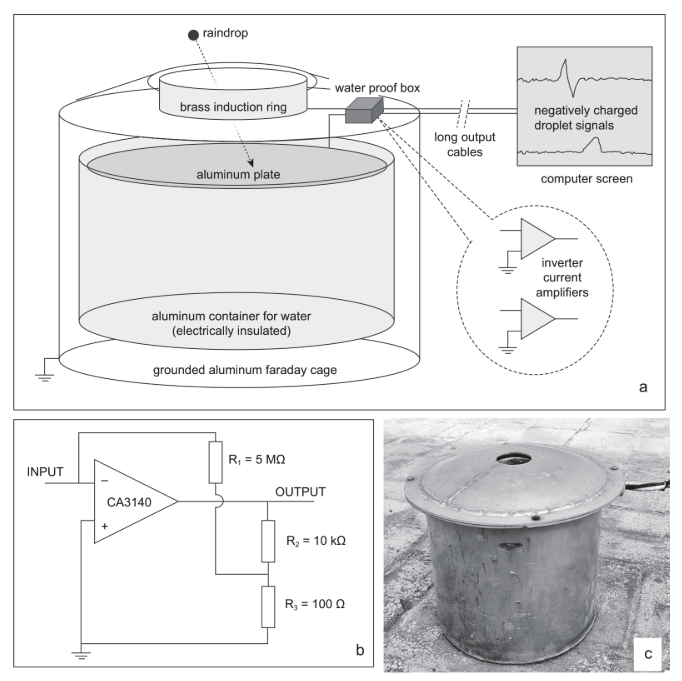
\includegraphics[width=0.7\textwidth]{figures/instrumento_de_medicion.png}
    \caption{(a) Diagrama del dispositivo de medición; (b) circuito amplificador inversor de corriente; (c) fotografía del dispositivo en el techo de la Facultad de Matemática, Astronomía, Física y Computación, Universidad Nacional de Córdoba.}
    \label{fig:instrumento_medicion}
\end{figure}

Los amplificadores están protegidos contra daños por agua al estar asegurados dentro de un recinto impermeable. La jaula de Faraday presenta una abertura ligeramente mayor que el anillo, permitiendo que las gotas de lluvia entren únicamente a través del anillo de inducción. Toda el agua que llega a la placa se drena a través de sus lados y se recolecta en un contenedor de aluminio, que también está situado dentro de la jaula de Faraday pero eléctricamente aislado de ella.

Las gotas cargadas eléctricamente inducen corrientes tanto en el anillo como en la placa. Al caer una gota, primero se acerca al anillo. Al hacerlo, se induce una corriente de la polaridad opuesta a la carga de la gota. Luego, al alejarse, esta polaridad se invierte. Mientras tanto, la gota se acerca a la placa, induciendo también una corriente de polaridad opuesta a la carga de la gota, lo cual culmina en una meseta en la corriente dado que la placa de aluminio absorbe el impacto de la gota y se le transfiere toda la carga a la placa, la cual se disipa en el tiempo. La figura \ref{fig:corriente_gotas} muestra la dinamica de este proceso con el registro de una gota.

\begin{figure}[!hb]
    \centering
    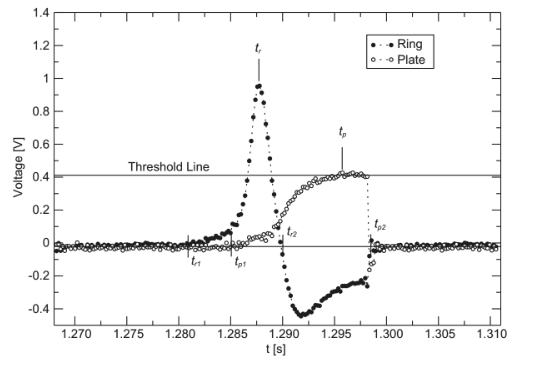
\includegraphics[width=0.7\textwidth]{figures/corriente_gotas.png}
    \caption{Corriente inducida por una gota cargada negativamente en el anillo (puntos solidos) y la placa (puntos huecos).}
    \label{fig:corriente_gotas}
\end{figure}

La adquisición de datos se realiza a una tasa de 5 kHz por canal (5000 datos por segundo). Por limitaciones de hardware, la adquisición de datos no se puede realizar al mismo tiempo que la escritura a disco, por lo que cada segundo se pierden $\sim$50ms de datos. Esto debe ser tenido en cuenta luego para analizar los datos obtenidos.

\subsection{Procesamiento de Señales}

El procedimiento de análisis de las señales consta de 5 pasos principales:

\begin{enumerate}
    \item Rellenado de huecos en los datos.
    \item Suavizado de las señales para quitar el ruido de fondo.
    \item Busqueda de picos en las señales.
    \item Aplicacion de filtros de calidad para extraer las gotas.
    \item Calculo de propiedades de las gotas.
\end{enumerate}

Para el procesamiento de los datos se han desarrollado dos programas en Fortran que trabajan de manera secuencial.

El primer programa se encarga del preprocesamiento de los datos, específicamente del rellenado de huecos mediante interpolación lineal y del suavizado de las señales para reducir el ruido de fondo.

El segundo programa realiza el análisis principal de las señales ya pre-procesadas. Implementa el algoritmo de detección de picos, aplica filtros para separar las gotas válidas, y calcula las propiedades físicas de ellas, incluyendo su tamaño, carga eléctrica y velocidad de caída.

\subsection{Necesidad de Mejoras}

El código actual, aunque funcional, sufre de varios problemas tanto en su diseño como en su rendimiento.

En primer lugar, el código consta de pocos archivos con una cantidad de líneas muy grande, lo que dificulta su mantenimiento y modificación. Cualquier cambio requiere revisar y entender todo el código, ya que las responsabilidades no están bien asignadas. Además, hay muchas variables sin nombres descriptivos y constantes hard-codeadas sin referencia alguna, lo que complica aún más la comprensión.

En segundo lugar, para grandes volúmenes de datos, la ejecución es muy lenta. Por ejemplo, para procesar datos de una tormenta de 5 horas de duración (aproximadamente 100M de datos), el programa requiere varias horas de ejecución. A esto se suma un consumo de memoria excesivamente alto, lo que obliga a procesar los datos de a partes. A su vez el algoritmo actual no tiene en cuenta las gotas que quedan en medio de estos cortes, resultando en la pérdida de algunos datos.

\subsection{Objetivos}

\subsubsection{Objetivo General}

Desarrollar un sistema modular y automatizado para el análisis de datos de gotas cargadas eléctricamente que mejore significativamente la eficiencia, mantenibilidad y escalabilidad del código existente, facilitando la obtención de nuevos resultados.

El nuevo sistema debe ser capaz de detectar mayor cantidad de gotas y debe ser capaz de procesar grandes volúmenes de datos de manera eficiente.

\subsubsection{Objetivos Específicos}

\begin{enumerate}
    \item \textbf{Diseñar una arquitectura modular} que separe las diferentes etapas del procesamiento en componentes independientes y reutilizables.
    
    \item \textbf{Implementar procesamiento paralelo} para analizar múltiples archivos de datos simultáneamente, reduciendo significativamente el tiempo total de procesamiento.
    
    \item \textbf{Desarrollar un sistema de automatización} que permita el procesamiento completo de conjuntos de datos sin intervención manual.
    
    \item \textbf{Optimizar el rendimiento} del algoritmo de detección de gotas para manejar grandes volúmenes de datos de manera eficiente.
    
    \item \textbf{Documentar completamente} el sistema para facilitar su uso por otros investigadores y su mantenimiento futuro.
\end{enumerate}

\subsection{Estructura de la Tesis}

Despues la hago

\section{Procedimiento}

\subsection{Análisis del Código Existente}

Aca iria el analisis de todo el codigo existente. Señalando todas las fallas especificas del codigo existente. Tambien habria que señalar el error que descubrimos en el llenado de huecos (que se hacia constante y no se hacia la interpolacion lineal).

\subsection{Algoritmos y estructuras de datos utilizadas}

Aca explicaria min-max-queue que lo uso para detectar los picos en O(1).

Tambien explicaria el algoritmo de promedio movil que uso para suavizar las señales.

Y capaz que me estoy olvidando de algo mas

\subsection{Implementación en C++}

Toda la explicacion del codigo de C++

\subsection{Sistema de Automatización}

Toda la explicacion del codigo de Python

\section{Resultados}

- Comparativas de tiempo
- Comparativas de memoria
- Comparativas de cantidad de gotas detectadas

Señalar todos los objetivos cumplidos en base a los planteados

\subsection{Limitaciones y Áreas de Mejora}

Despues vemos

\section{Conclusiones}

Veremos 

\section{Referencias}

\begin{enumerate}
    \item Despues las hago
\end{enumerate}

\end{document}
